\begin{figure}[htbp]
\centering
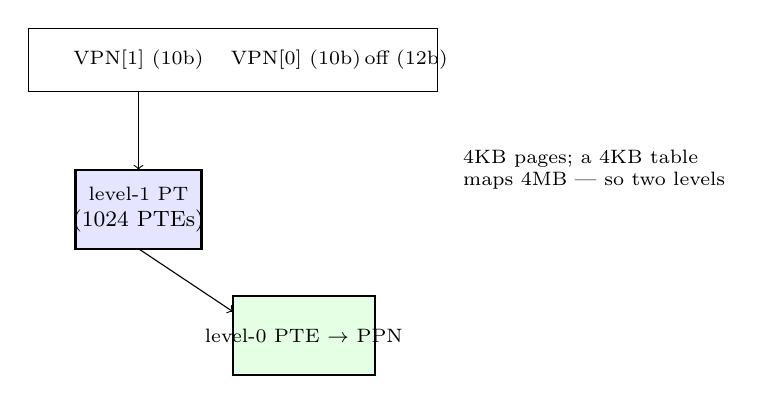
\begin{tikzpicture}[font=\footnotesize, x=1cm, y=1cm]
  \draw (0,3.6) rectangle (5.2,4.4);
  \node at (1.4,4.0) {\scriptsize VPN[1] (10b)};
  \node at (3.4,4.0) {\scriptsize VPN[0] (10b)};
  \node at (4.8,4.0) {\scriptsize off (12b)};
  \draw[->] (1.4,3.6) -- (1.4,2.6);
  \draw[thick,fill=blue!10] (0.6,1.6) rectangle (2.2,2.6);
  \node[align=center] at (1.4,2.1) {\scriptsize level-1 PT\\ (1024 PTEs)};
  \draw[->] (1.4,1.6) -- (2.6,0.8);
  \draw[thick,fill=green!10] (2.6,0.0) rectangle (4.4,1.0);
  \node at (3.5,0.5) {\scriptsize level-0 PTE $\to$ PPN};
  \node[anchor=west,align=left,font=\scriptsize] at (5.4,2.6)
    {4KB pages; a 4KB table\\ maps 4MB --- so two levels};
\end{tikzpicture}
\caption{The sv32 walk: VA[31:22] indexes the level-1 table for a
second-level table's physical address; VA[21:12] indexes that for
the PPN. Two memory reads per miss --- which is why the TLB exists.}
\label{fig:sv32_11}
\end{figure}
